\documentclass[a4paper, 10pt]{article}
\usepackage[utf8]{inputenc} % Change according your file encoding
\usepackage{graphicx}
\usepackage{url}

%opening
\title{Seminar Report: Muty}
\date{\normalsize\today{}}

\begin{document}

\maketitle

\begin{center}
  \textbf{Carles Tornel}\\
  \textbf{Jesus Alfaro}\\
  \textbf{Ricard Abril}

\end{center}

\section{Introduction}

\newpage
\section{Experiments}
\paragraph[bold]{Some Testing}
\begin{enumerate}
\item Make tests with different Sleep and Work parameters to analyze how this lock implementation responds to different contention degrees.
\paragraph[bold]{Test 1: Sleep time inferior a work time\\\\}
Si el temps de sleep és considerablement més petit que el temps de work, la probabilitat de que diferents workers demanin accés a la regió critica serà més alta, quan això passa, aquets workers esperaran un missatge d' OK de la resta, però aquets també es estaran en la mateixa situació, de forma que ens trobarem davant d'un deadlock. Encara que al estar durant 8 segons en aquesta situació, el programa allibera els lock, per tal de poder seguir executant-se. Tal i com podem veure en la següent imatge:\\\\
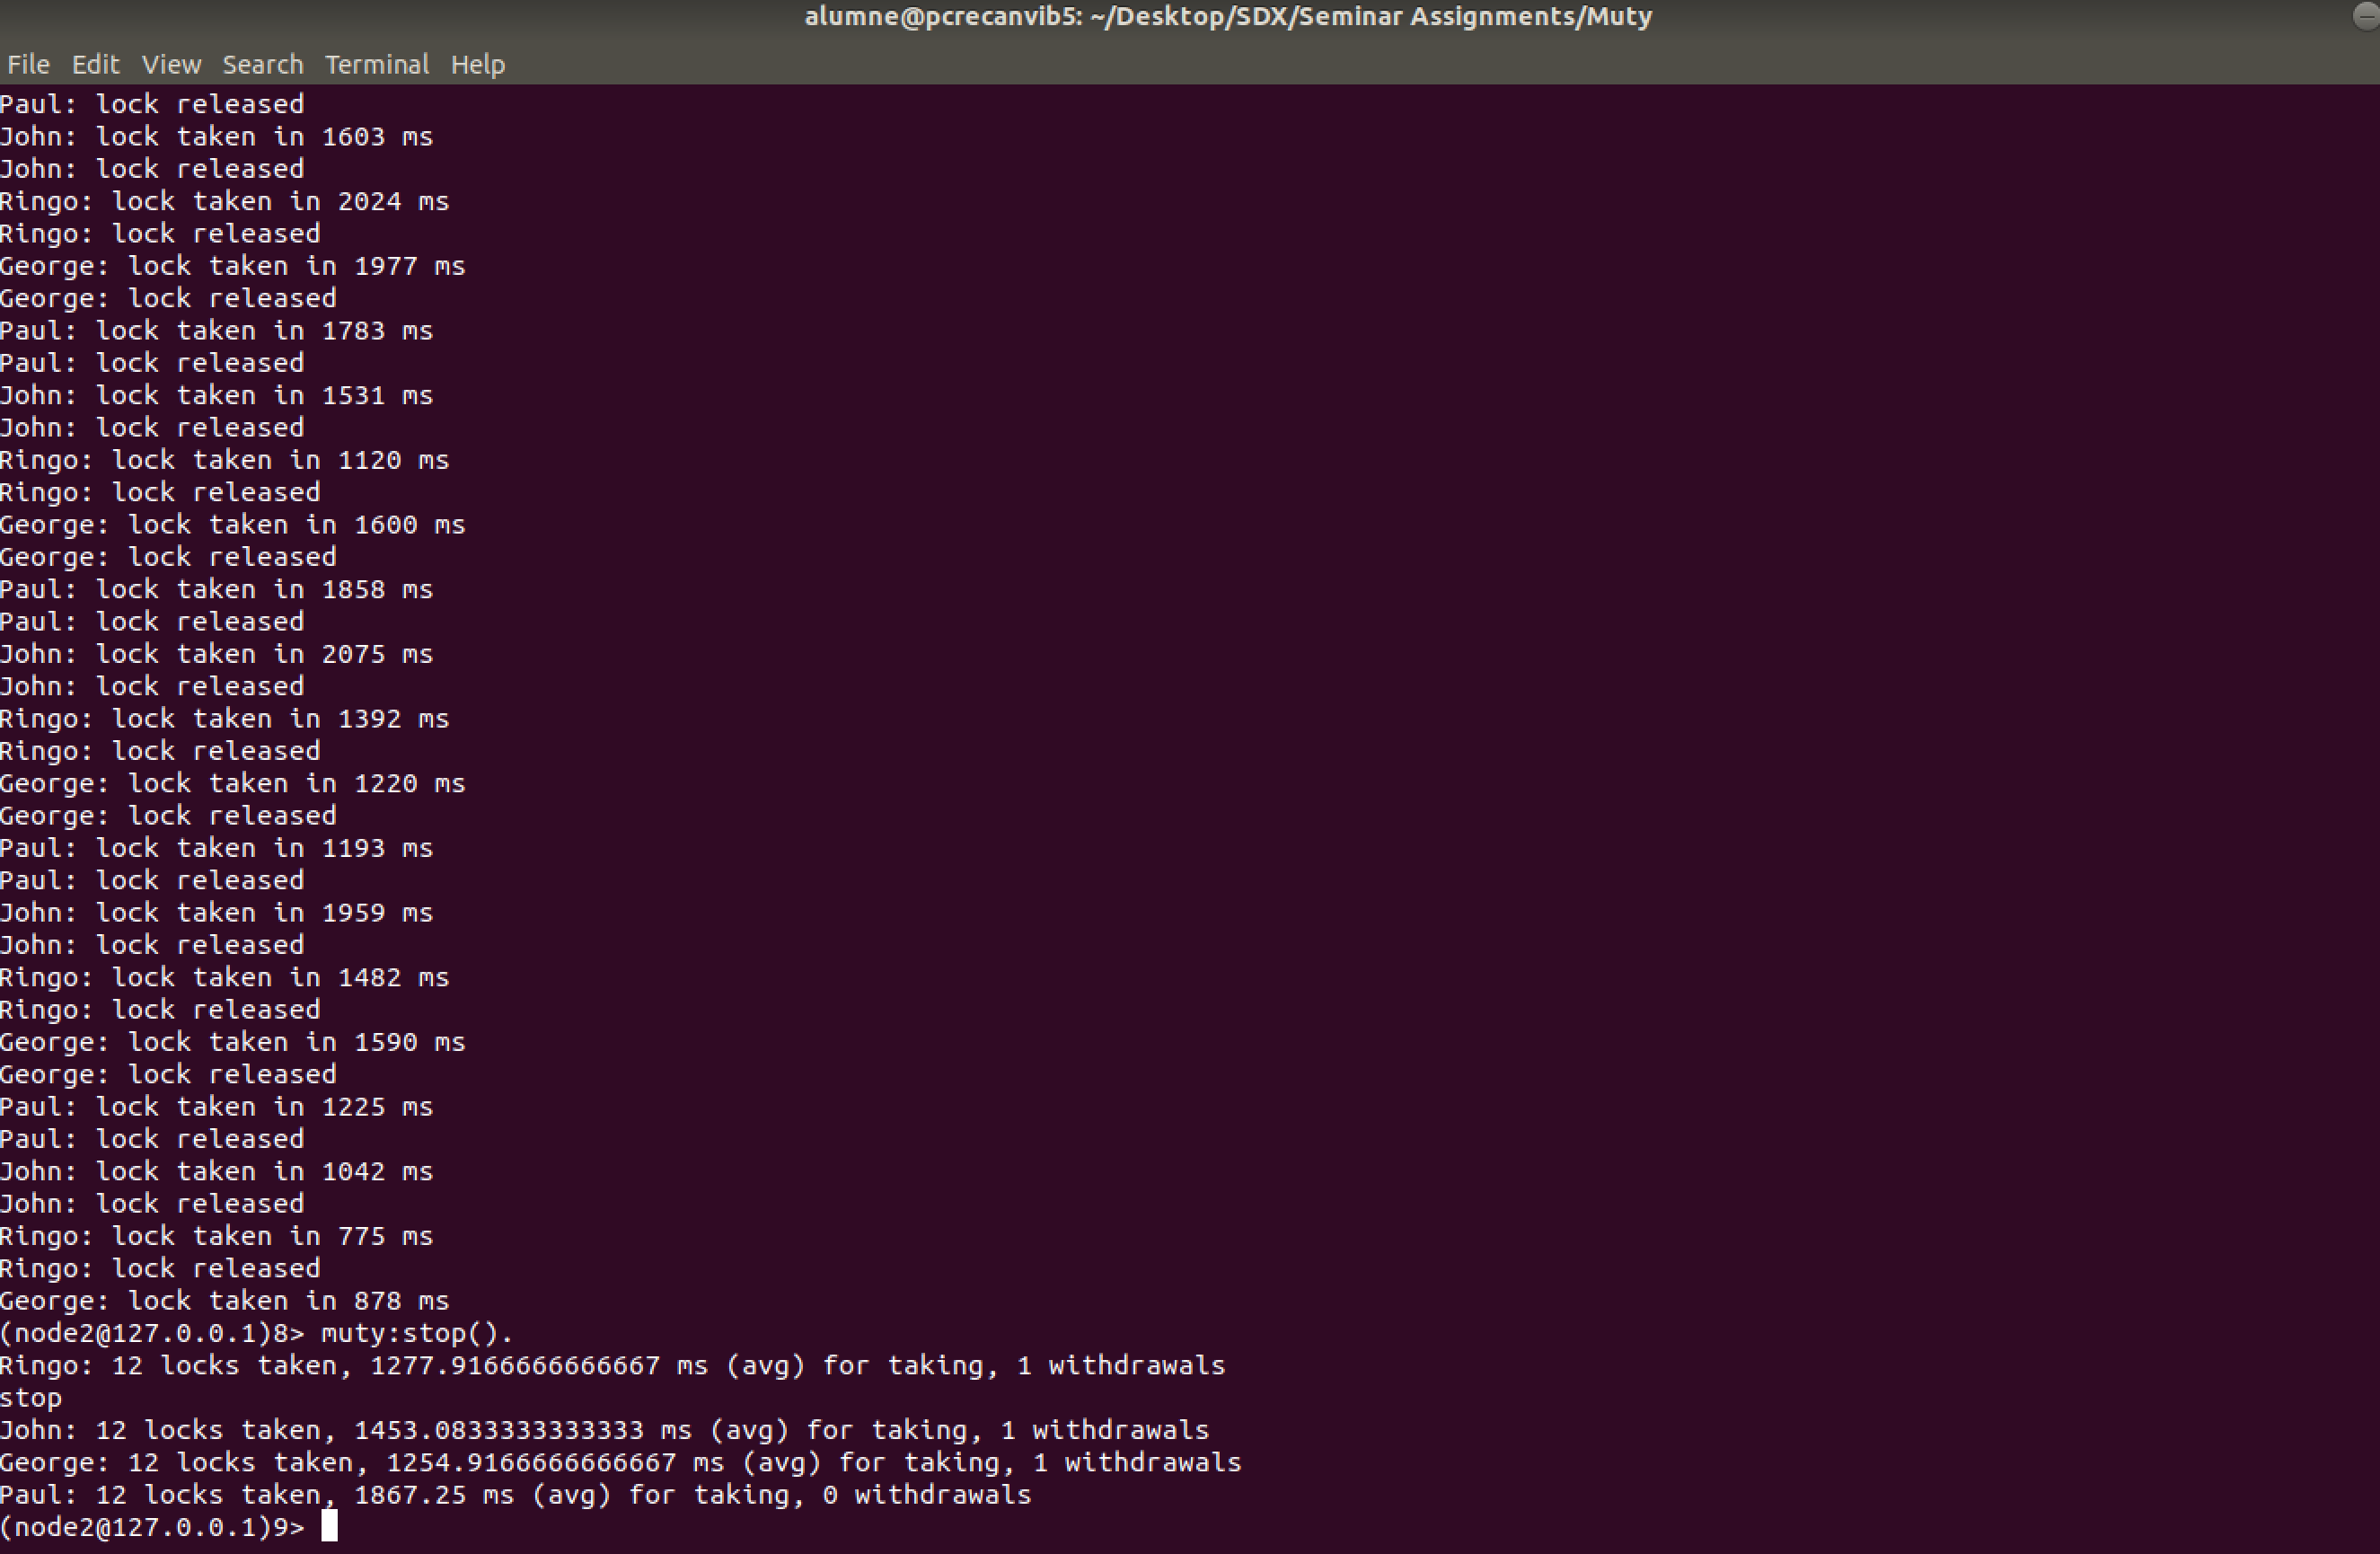
\includegraphics[width=\textwidth]{test-1}
\newpage També ens podem trobar amb la situació de que el temps de work, sigui més gran que el withdrawal time, per tant els workers a la espera superarien aquet temps. Tal i com podem observar:\\\\
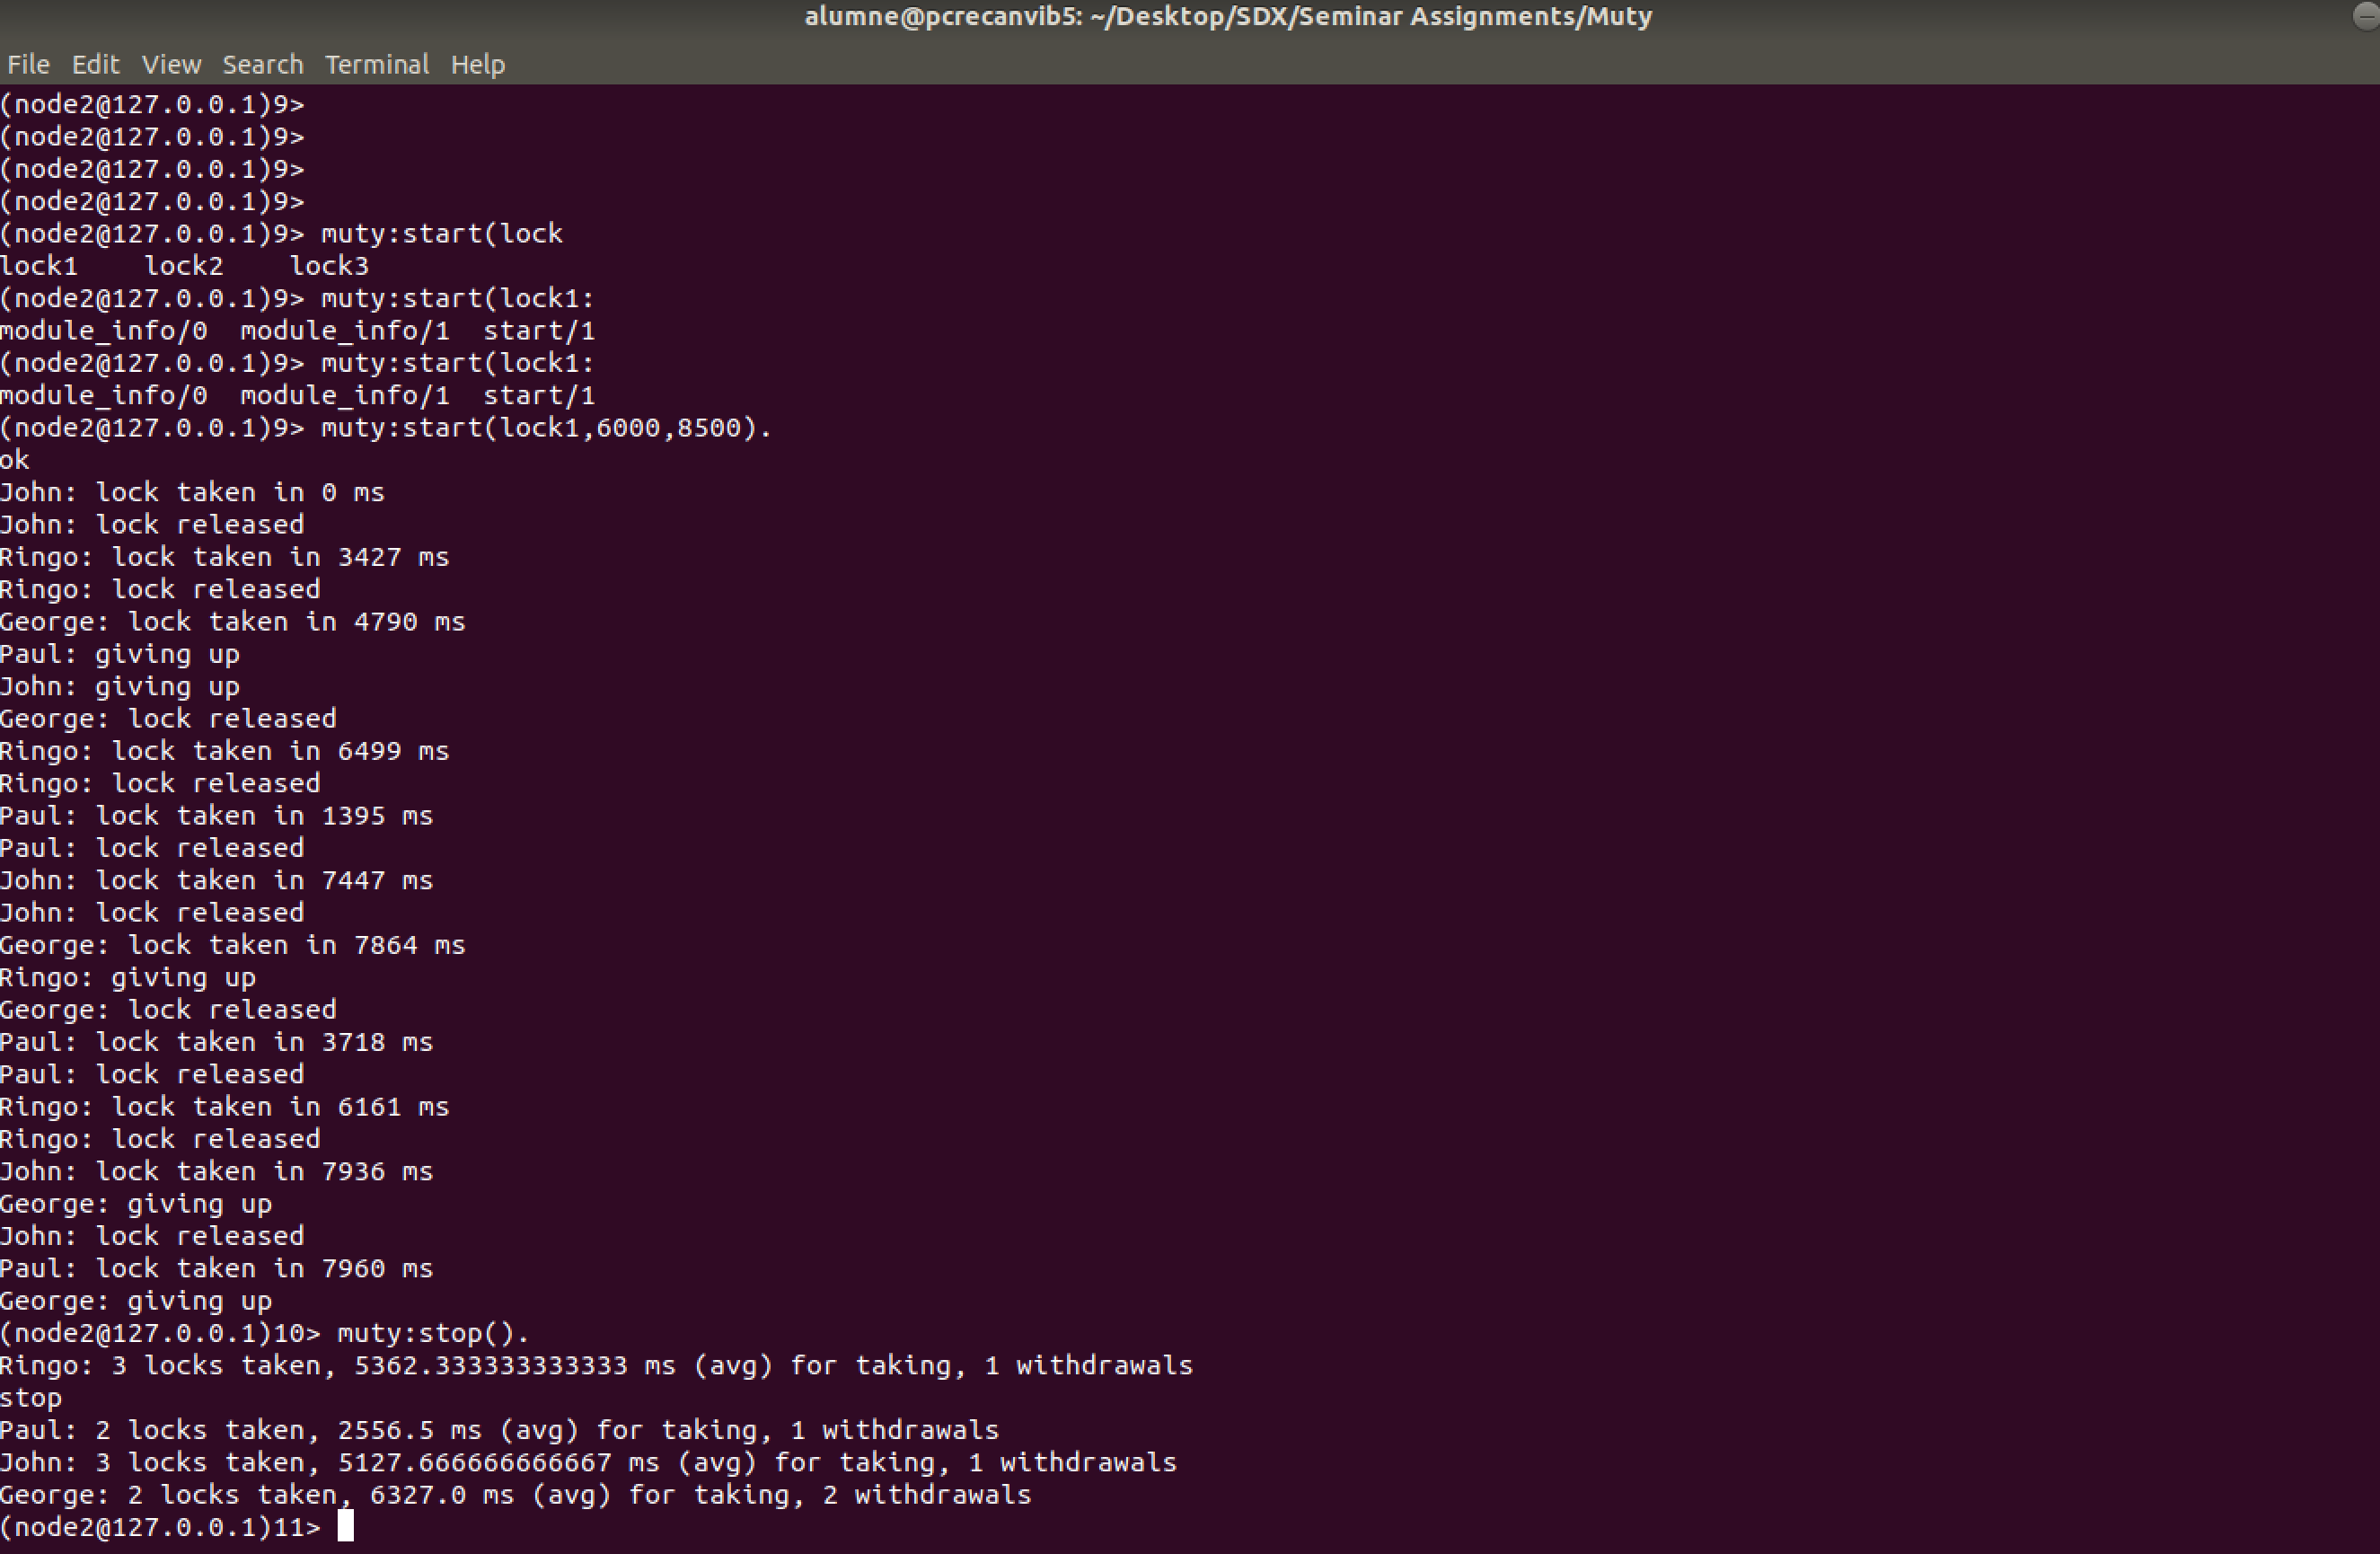
\includegraphics[width=\textwidth]{test-2}
\newpage\paragraph[bold]{Test 2: Sleep time superior a work time\\\\}
Si el temps de sleep, és més gran que el temps de work, estarem provocant, que les peticions d’accés a la regió critica dels diferents workers, estigui més espatllada, i per tant la possibilitat de trobar-nos en una situació de deadlock serà més baixa. Encara que no es una solució definitiva, ja que encara que essent menys probable també ens podem trobar amb una situació de deadlock, tal i com podem observar en la següent imatge:\\

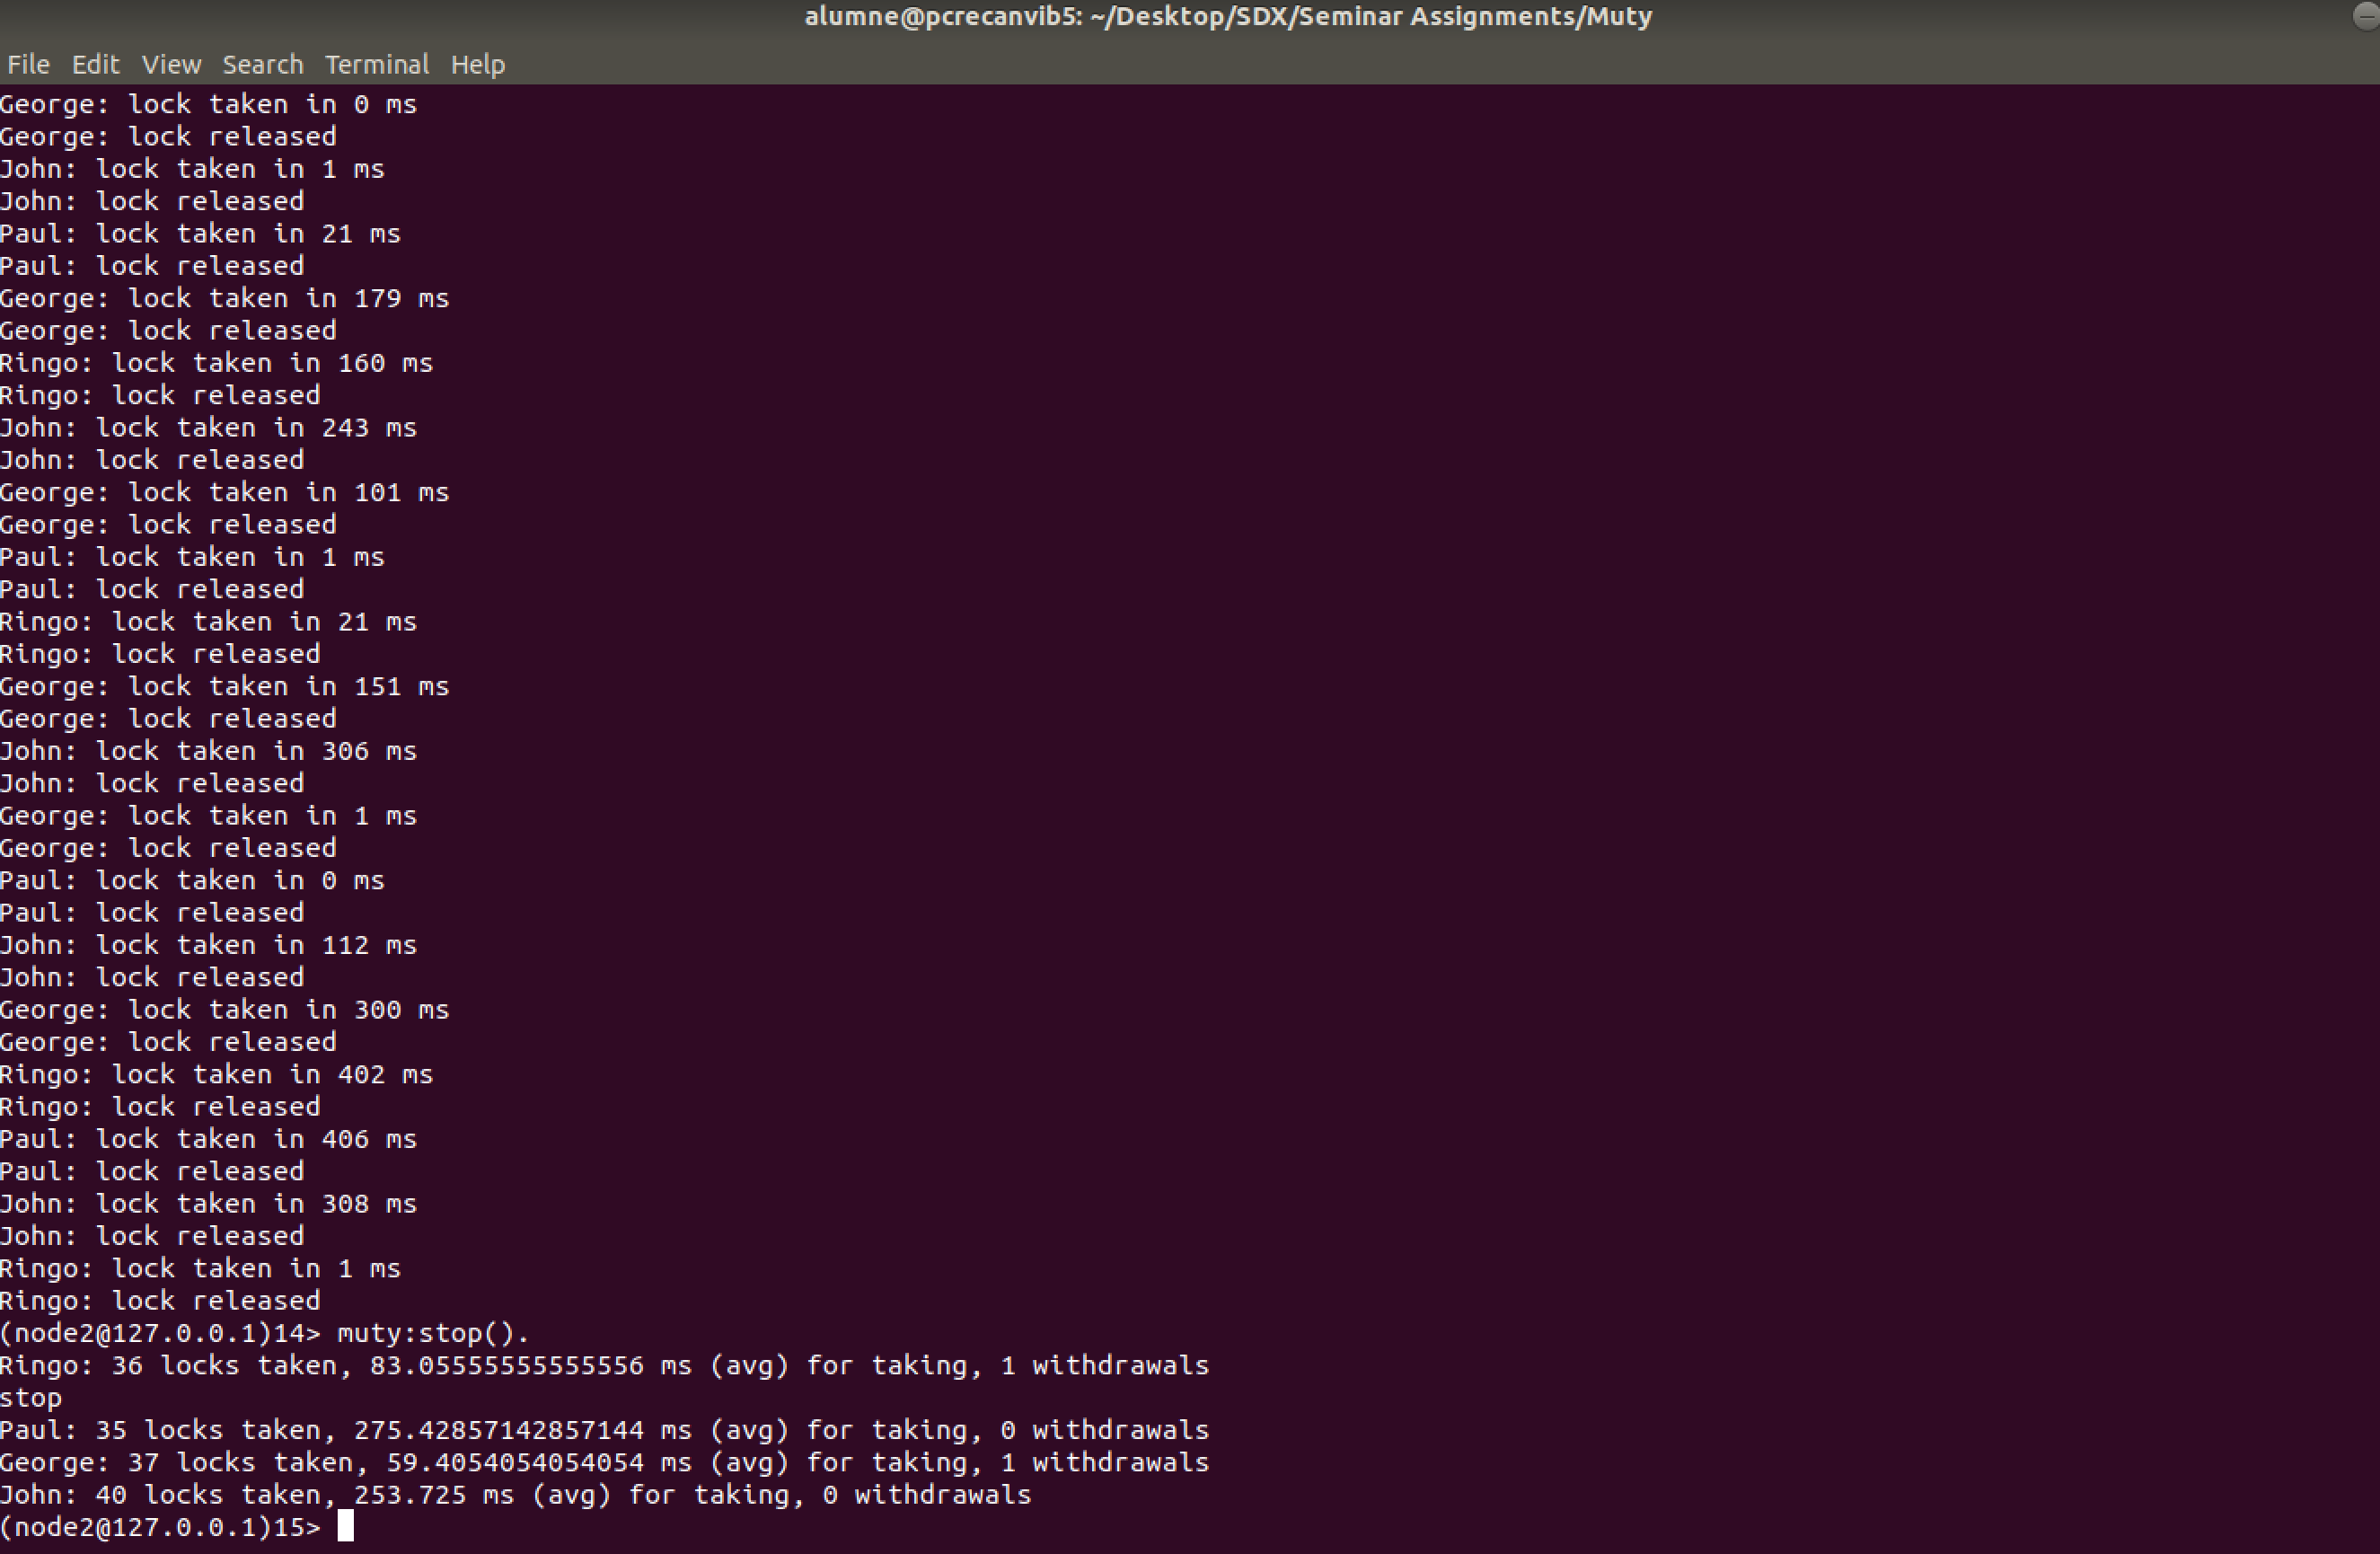
\includegraphics[width=\textwidth]{test-3}
\newpage
\paragraph[bold]{Test 3: Sleep time i work time iguals\\\\}

En aquesta situació, a la llarga també ens podriem trobar amb deadlocks, encara que  seran improbables com quan el sleep time es menor al work time. Ho podem observar en la següent imatge:\\

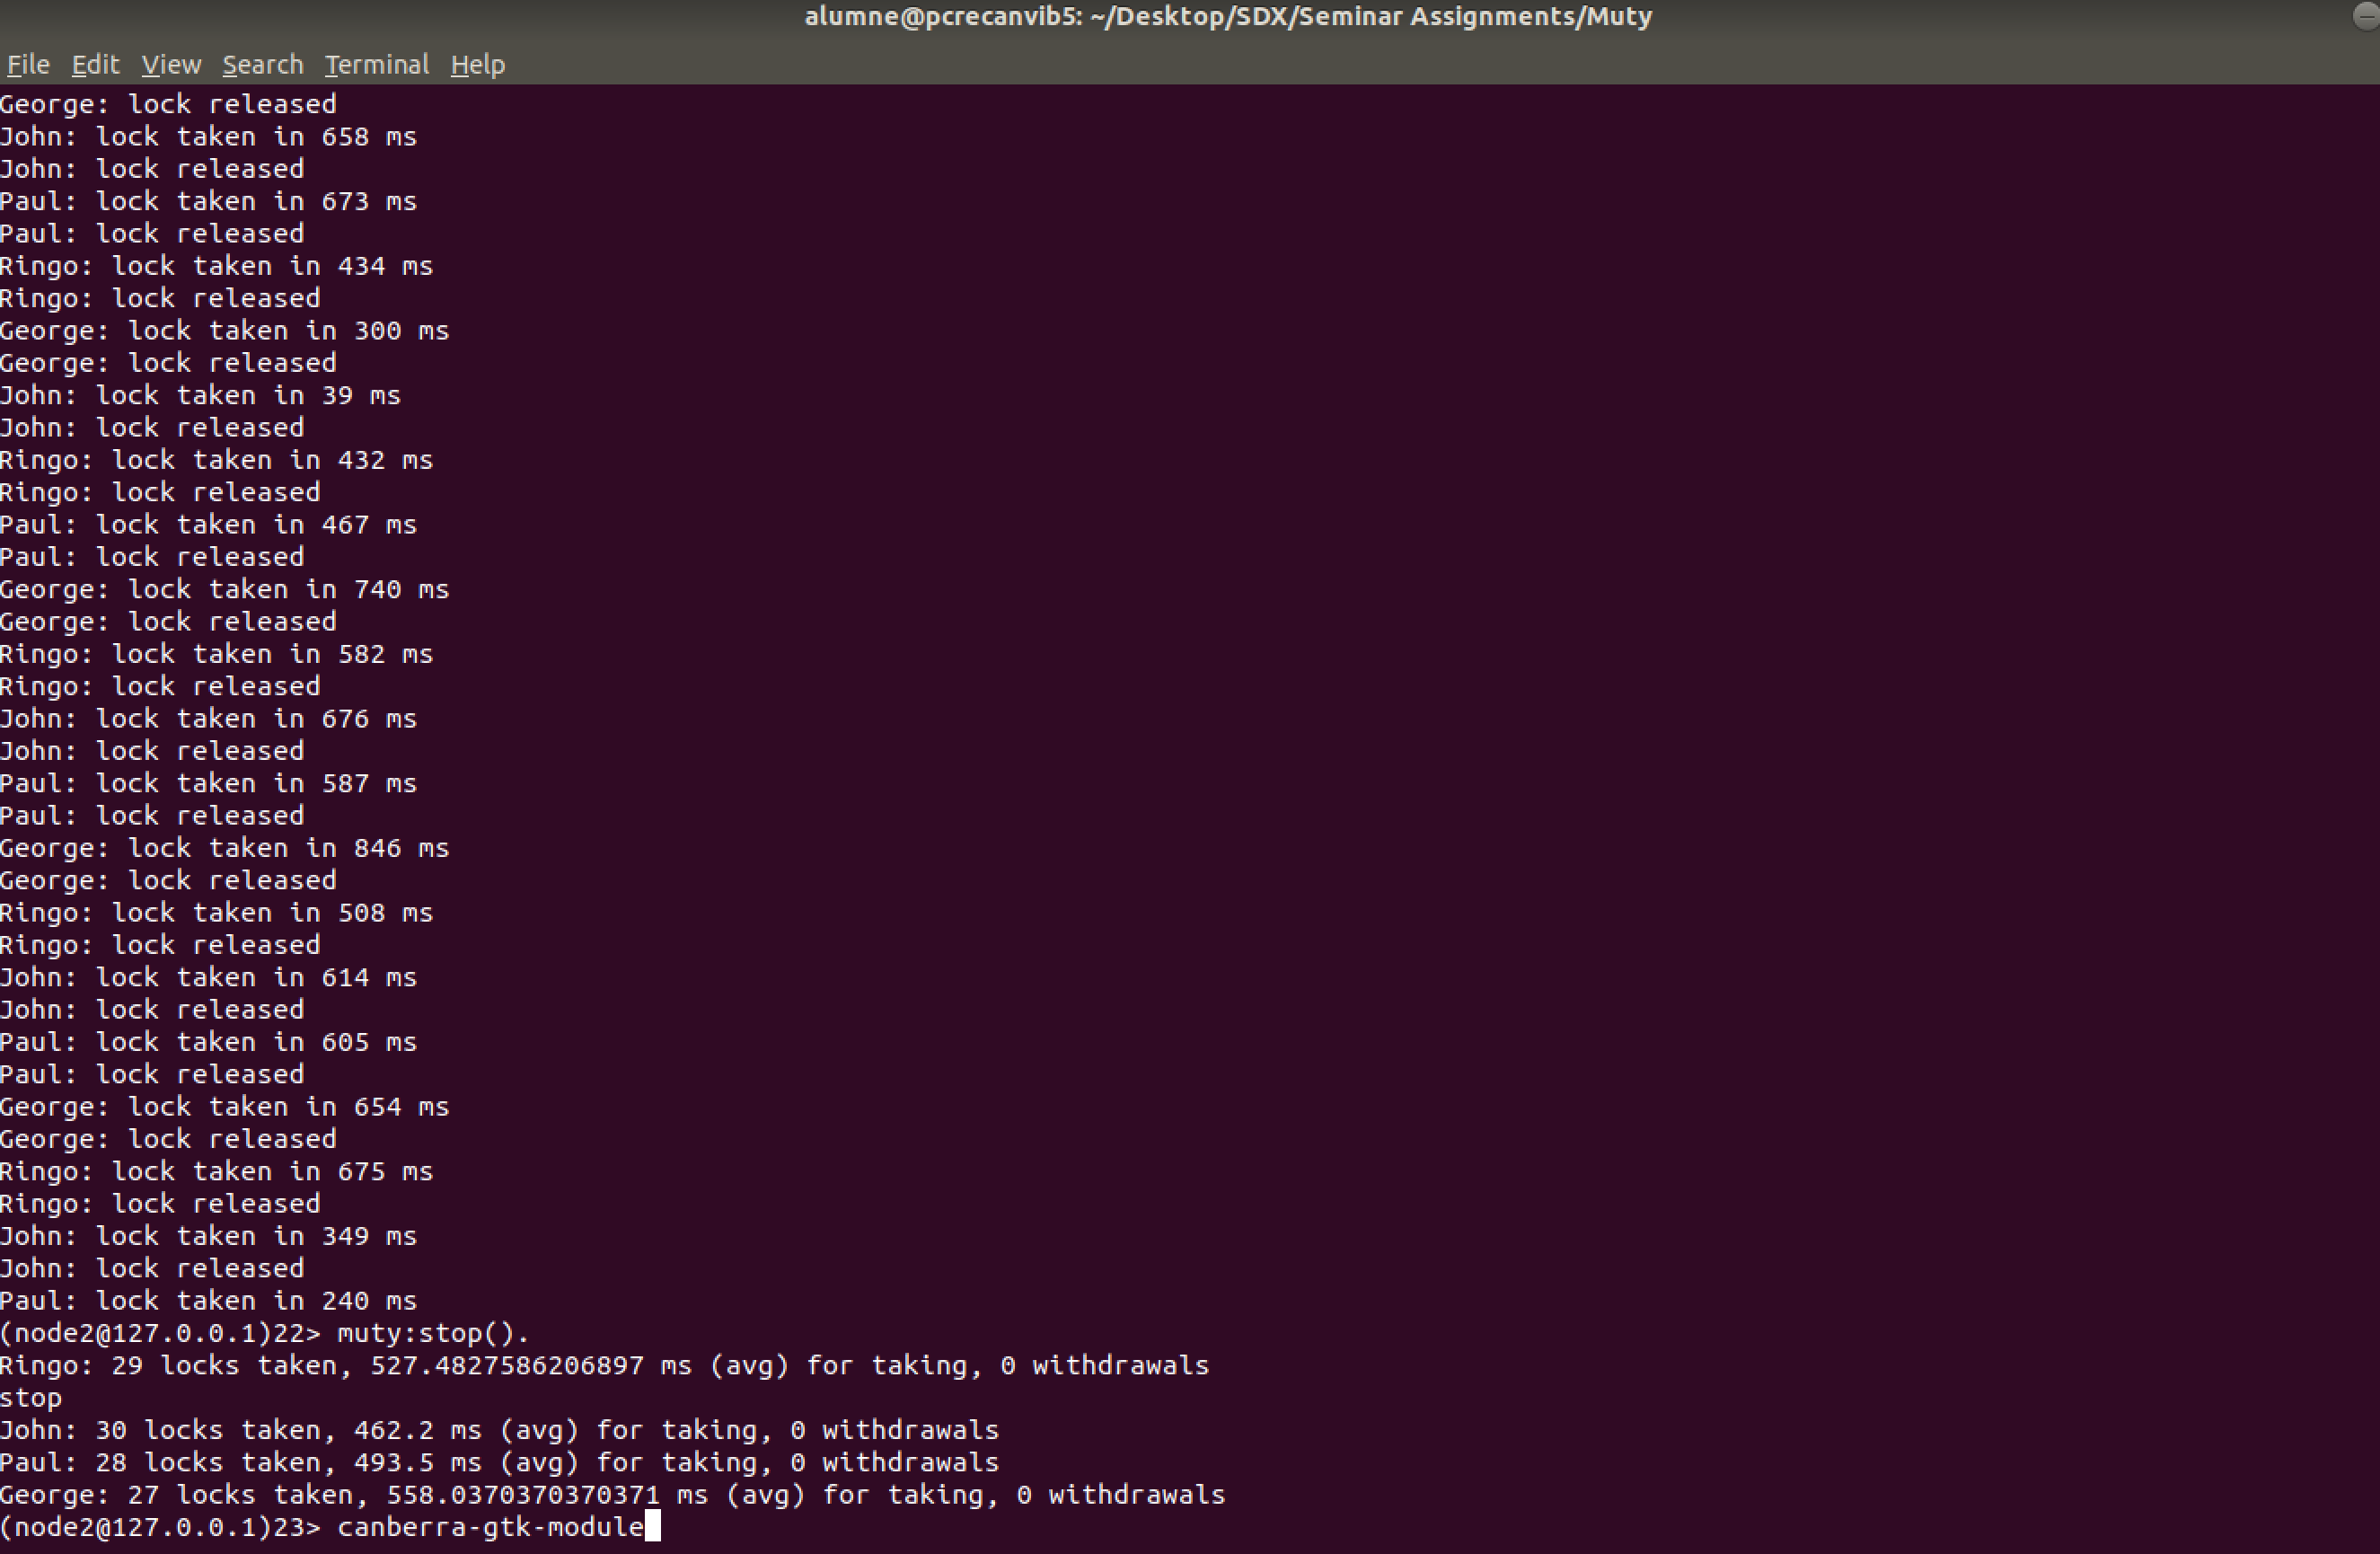
\includegraphics[width=\textwidth]{test-4}
\item Adapt the muty module to create each worker-lock pair in a different Erlang instance (that is, john and l1 should run in a node, ringo and l2 in another, and so on). Remember how processes are created remotely, how names registered in remote nodes are referred, and how Erlang runtime should be started to run distributed programs.\\\\

En la imatge següent podem veure les modificacions en el fitxer muty, per a que inici els workers en diferents instàncies de erlang\\\\

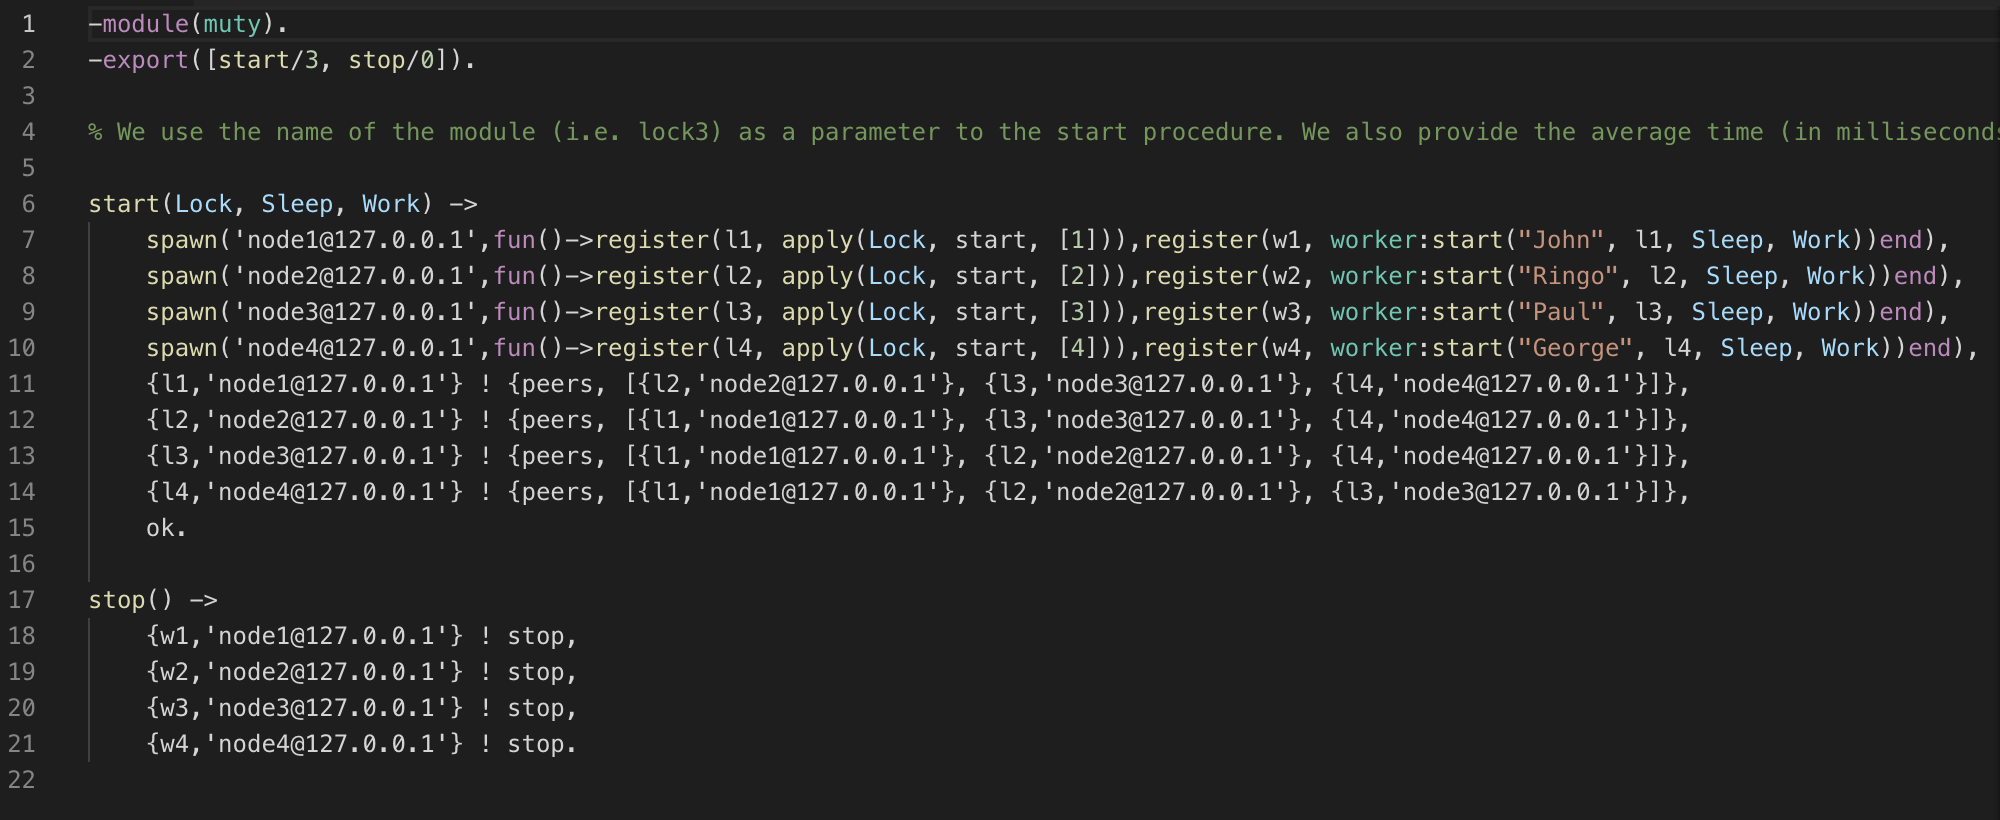
\includegraphics[width=\textwidth]{muty-code}

Tal i com podem veure en la imatge, els diferents workers s'executen en instàncies de erlang diferents.\\\\

\includegraphics[width=\textwidth]{muty-work}

\end{enumerate}

\newpage\paragraph[bold]{Resolving deadlock}
\begin{enumerate}
\item Repeat the previous tests to compare the behavior of this lock with respect to the previous one.
\paragraph[bold]{Test 1: Sleep time inferior a work time}

Per evitar els deadlocks, ara en cas de que diversos workers vulguin accedir a la regió critica del codi al mateix temps, el worker amb el ID més petit serà el que rebrà el missatge OK i podrà accedir. Amb aquet sistema evitarem els deadlocks, encara que el repartiment de feina, no serà massa equitatiu, ja que els workers amb ID més petit sempre tindran més prioritat, i per tant en cas de "empat", sempre acabaran fent la feina. Això ho podem observar en la següent imatge:\\\\

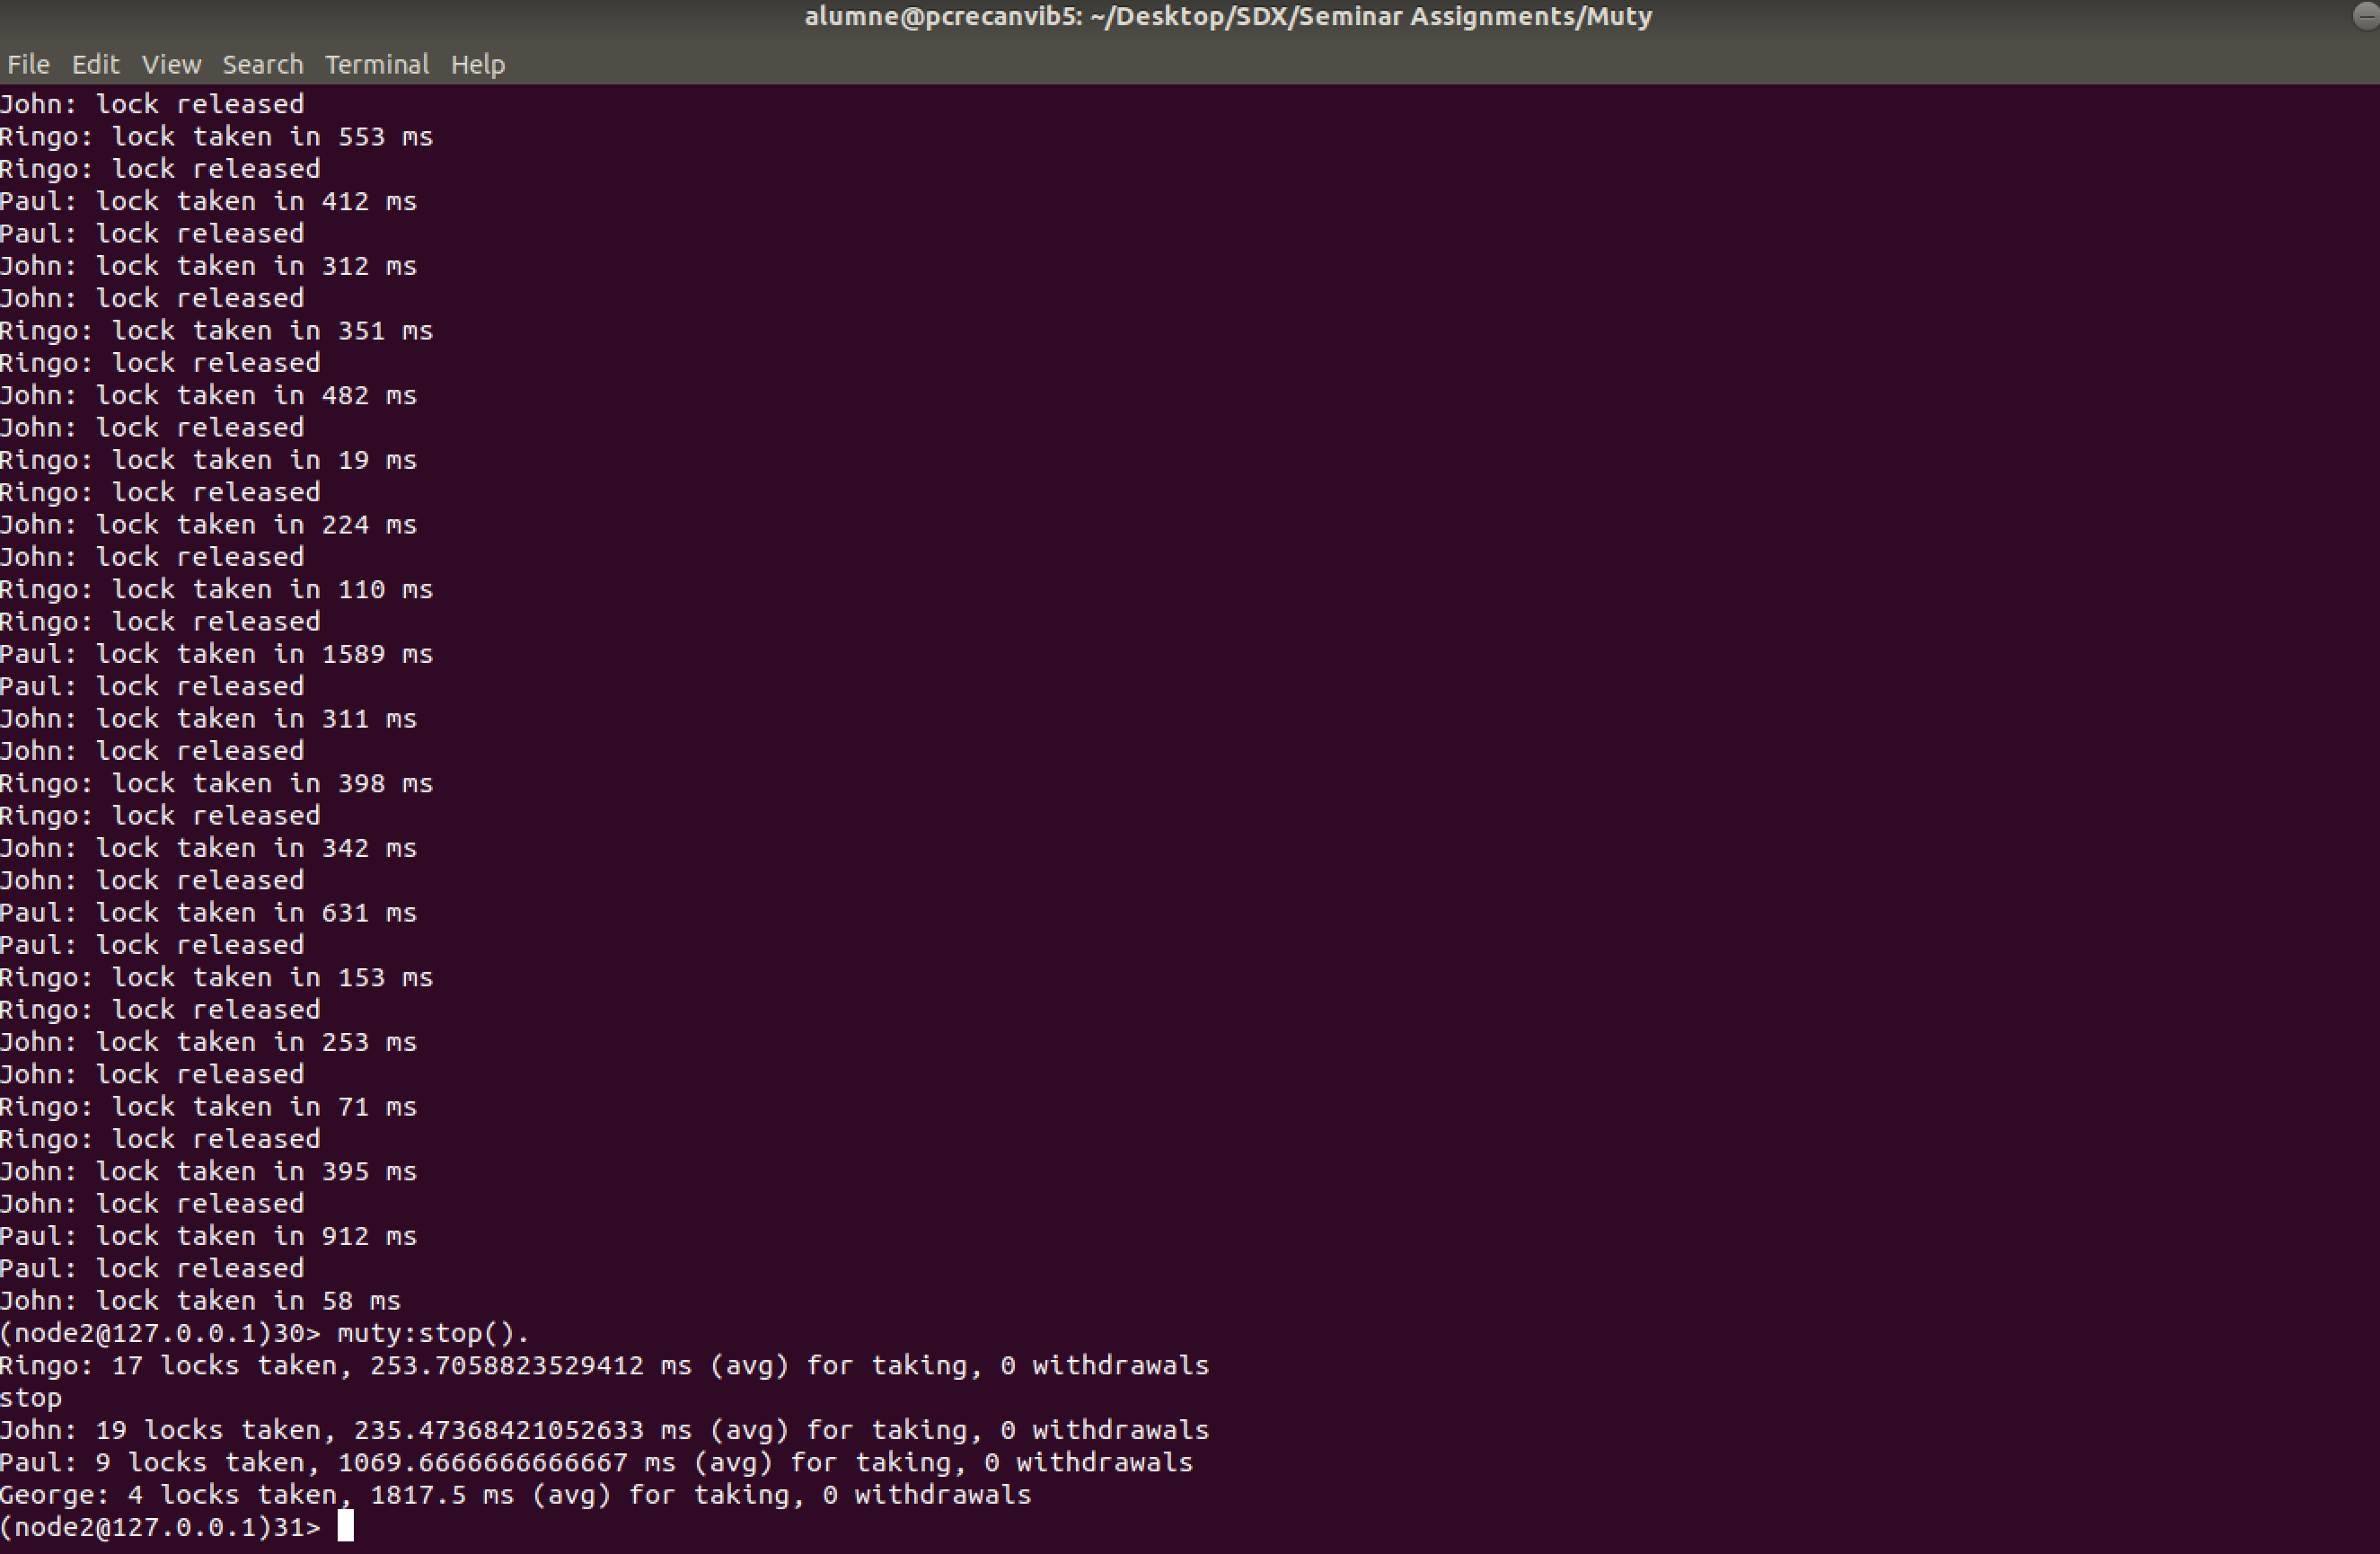
\includegraphics[width=\textwidth]{lock-1}
\newpage


\paragraph[bold]{Test 2: Sleep time superior a work time}

En aquesta situació, al tenir un sleep time major al work time, la probabilitat de que dos workers intentin accedir a la regió critica al mateix temps es redueix, per tant el repartiment de feina serà més equitatiu, encara que dista de ser perfecte. Podem observar-ho a la següent imatge:\\\\

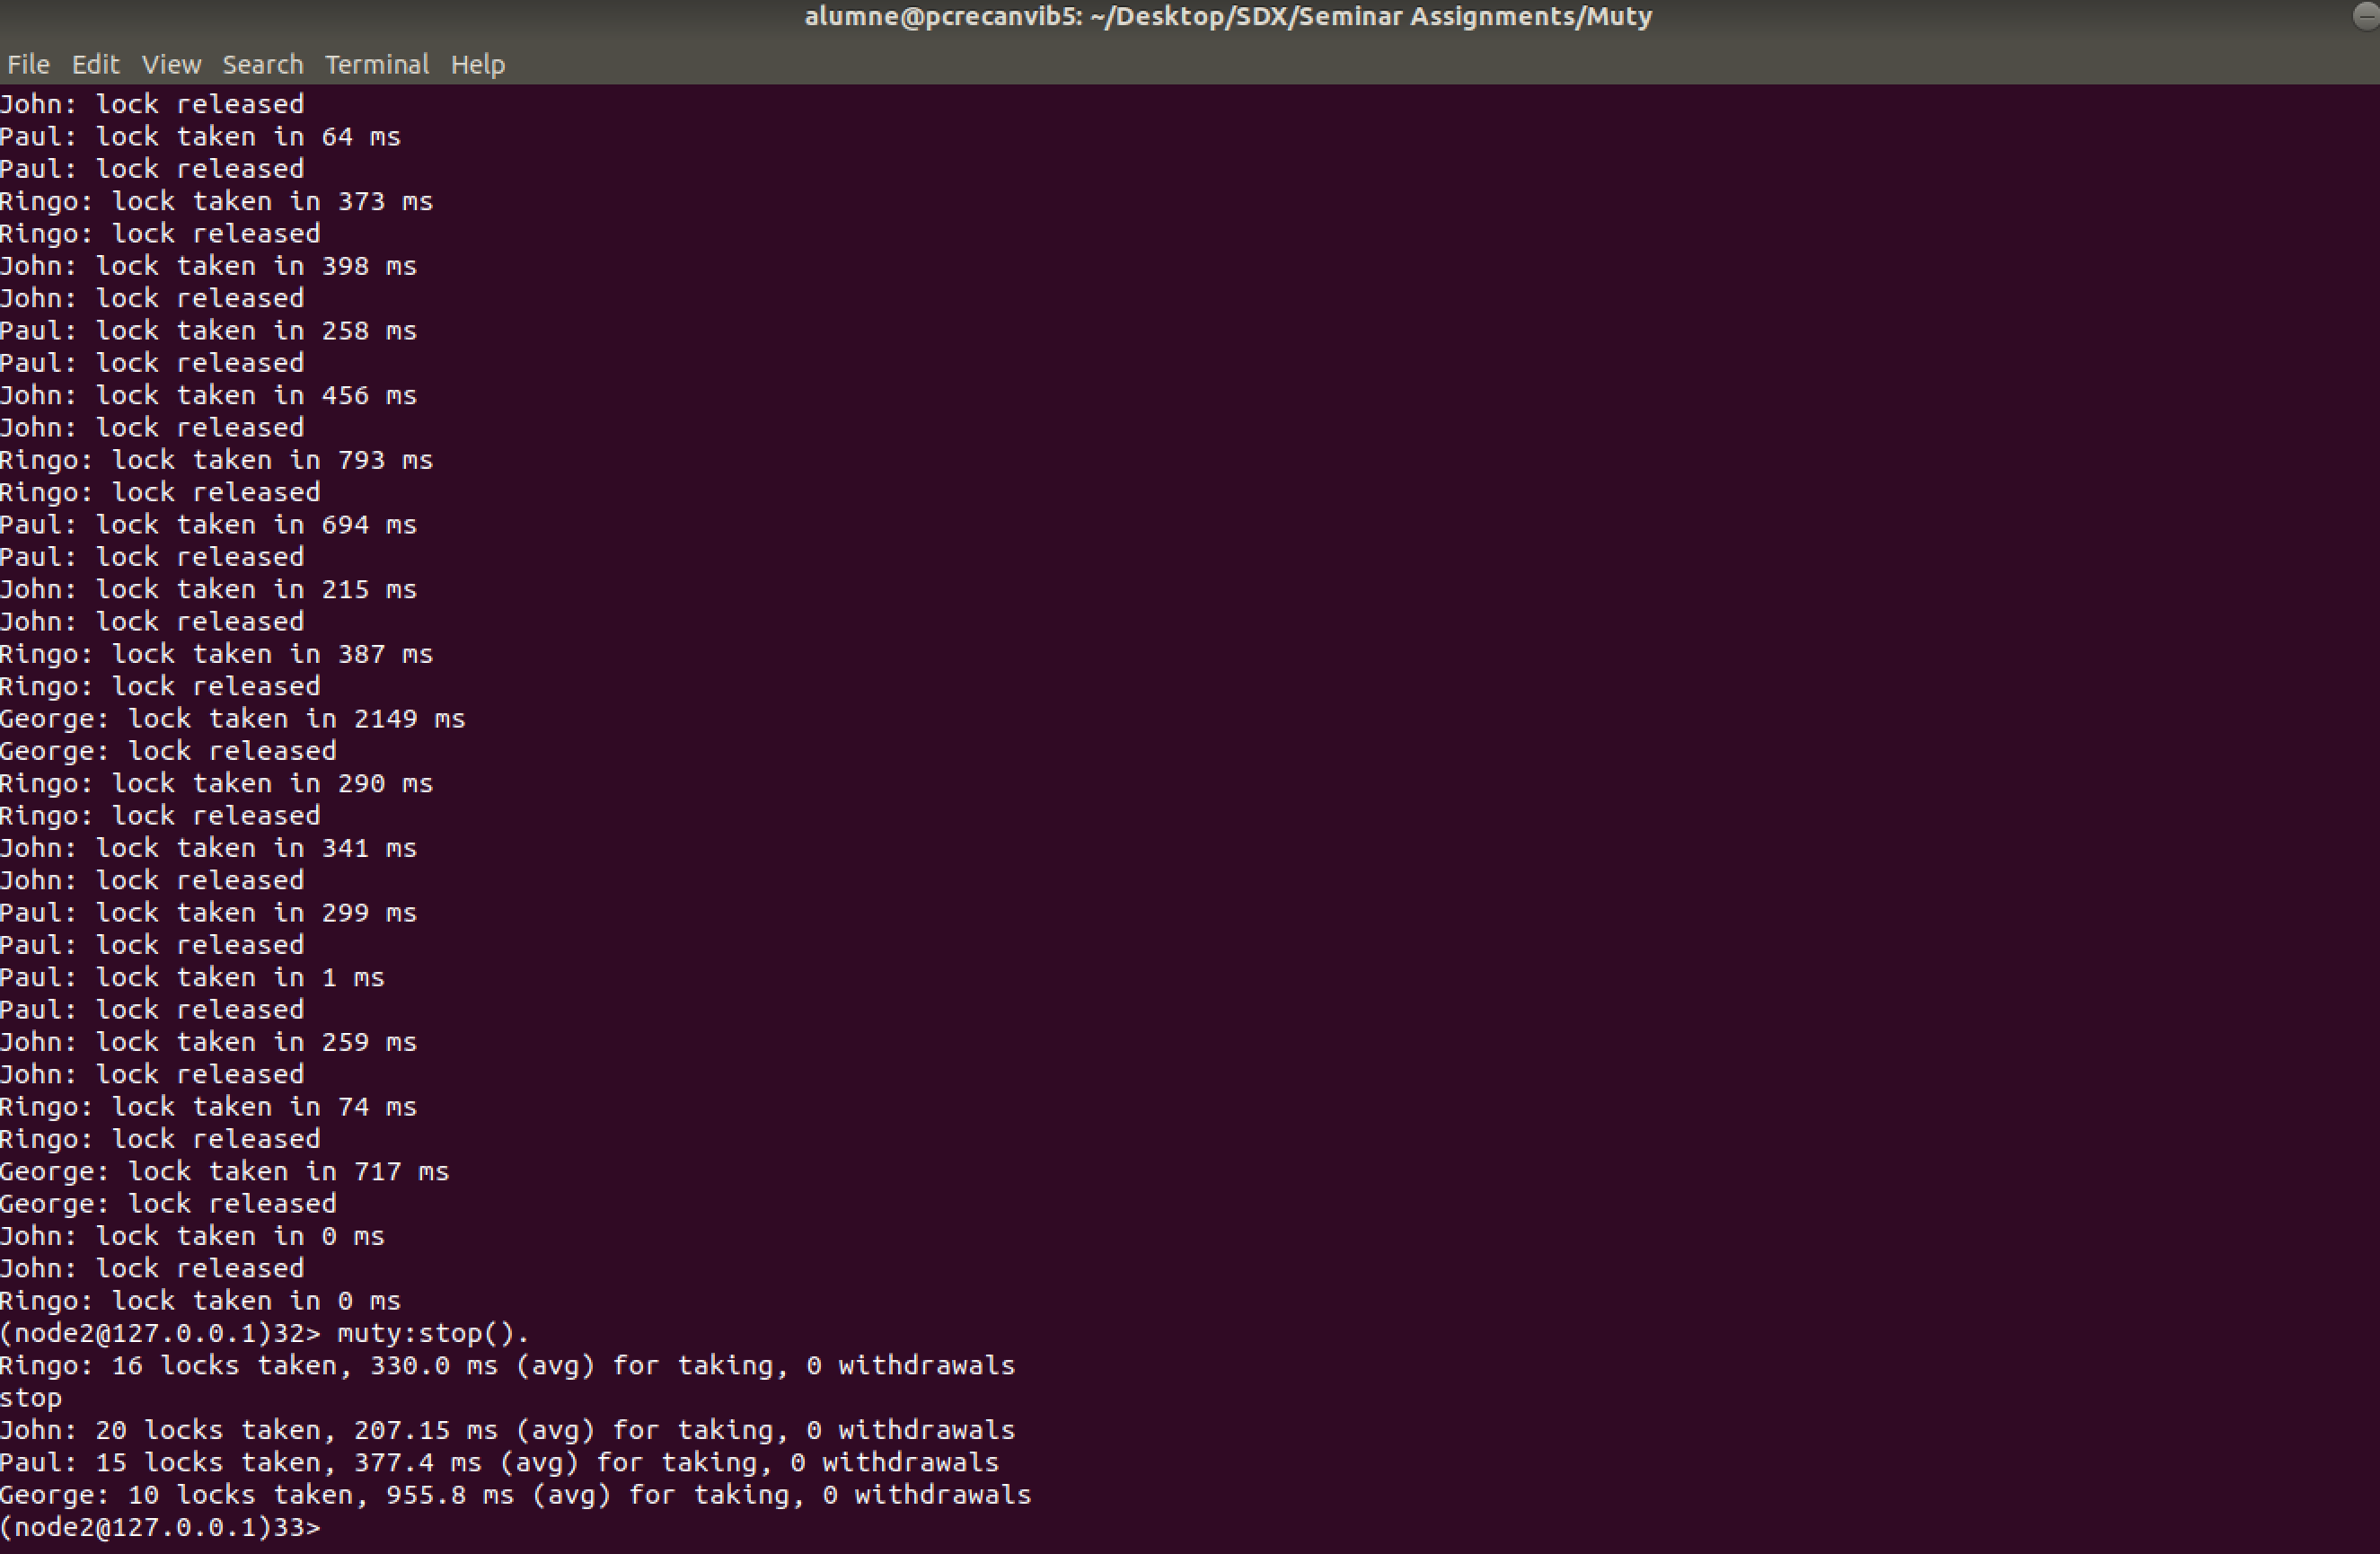
\includegraphics[width=\textwidth]{lock-2}
\\\\En aquet cas, ja no cal fer l'experiment per el cas de que el work time sigui igual al sleep time, ja que el resultat serà el mateix.

\end{enumerate}

\newpage
\paragraph[bold]{Lamport’s time}
\begin{enumerate}
\item Repeat the previous tests to compare this version with the former ones.
\paragraph[bold]{Test 1: Sleep time inferior a work time\\\\}
En aquet cas, per millorar la implementació anterior, hem aplicat el algorisme de Lamport, que ens permetrà un millor repartiment de la feina.
Això es degut a que en el moment que dos workers demanin accés a la regió critica, el que tingui el clock més petit, serà el que accedirà, no el que tingui el ID més petit. Per altra banda, en cas de que el temps de work sigui molt mes gran que el temps de sleep, els workers poden enviar missatges de release. Tal i com podem observar en la següent imatge:\\\\

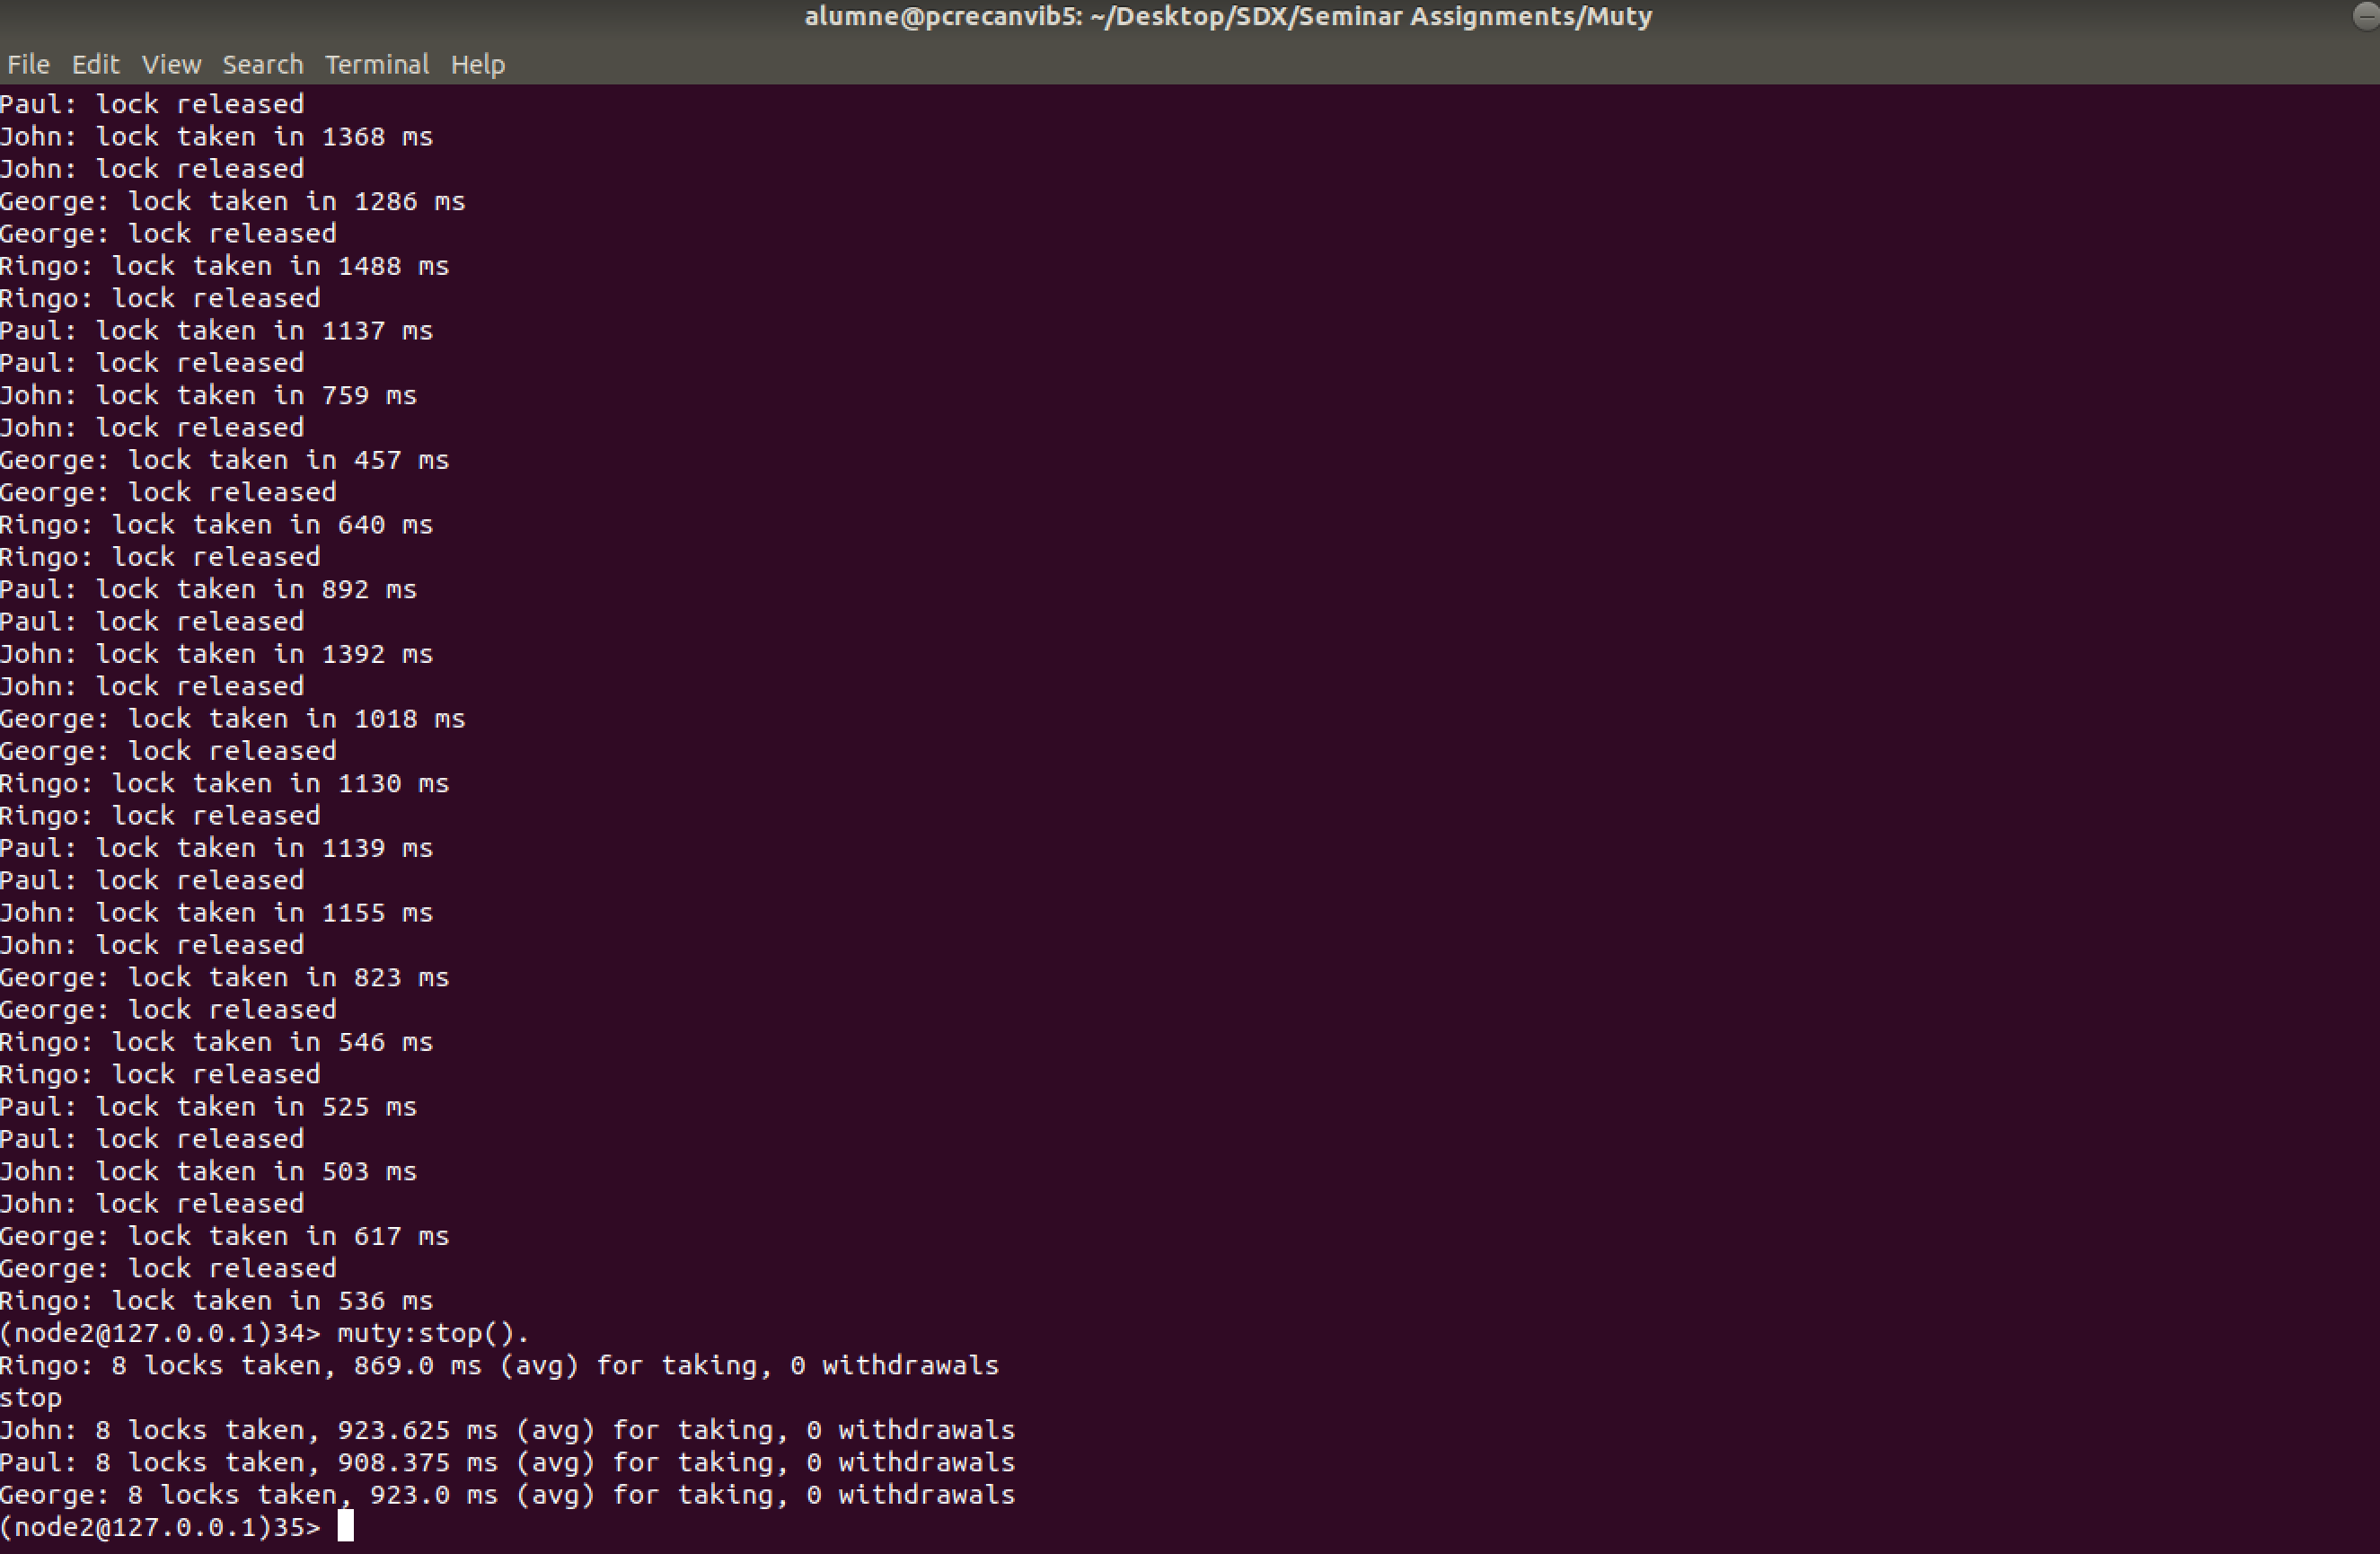
\includegraphics[width=\textwidth]{lamp-1}

Per altra part, tal i com passa en la secció anterior, si el temps de work és més gran que el temps de withdrawal, hi haurà workers, que no seran capaços de accedir a la regió critica.

\newpage
\paragraph[bold]{Test 2: Sleep time superior a work time\\\\}


En el cas de que el sleep time sigui més gran que el work time, els workers, no tindran problema per accedir a la regió critica, ja que com podem observar en la següent imatge el temps de lock és pràcticament 0.\\\\


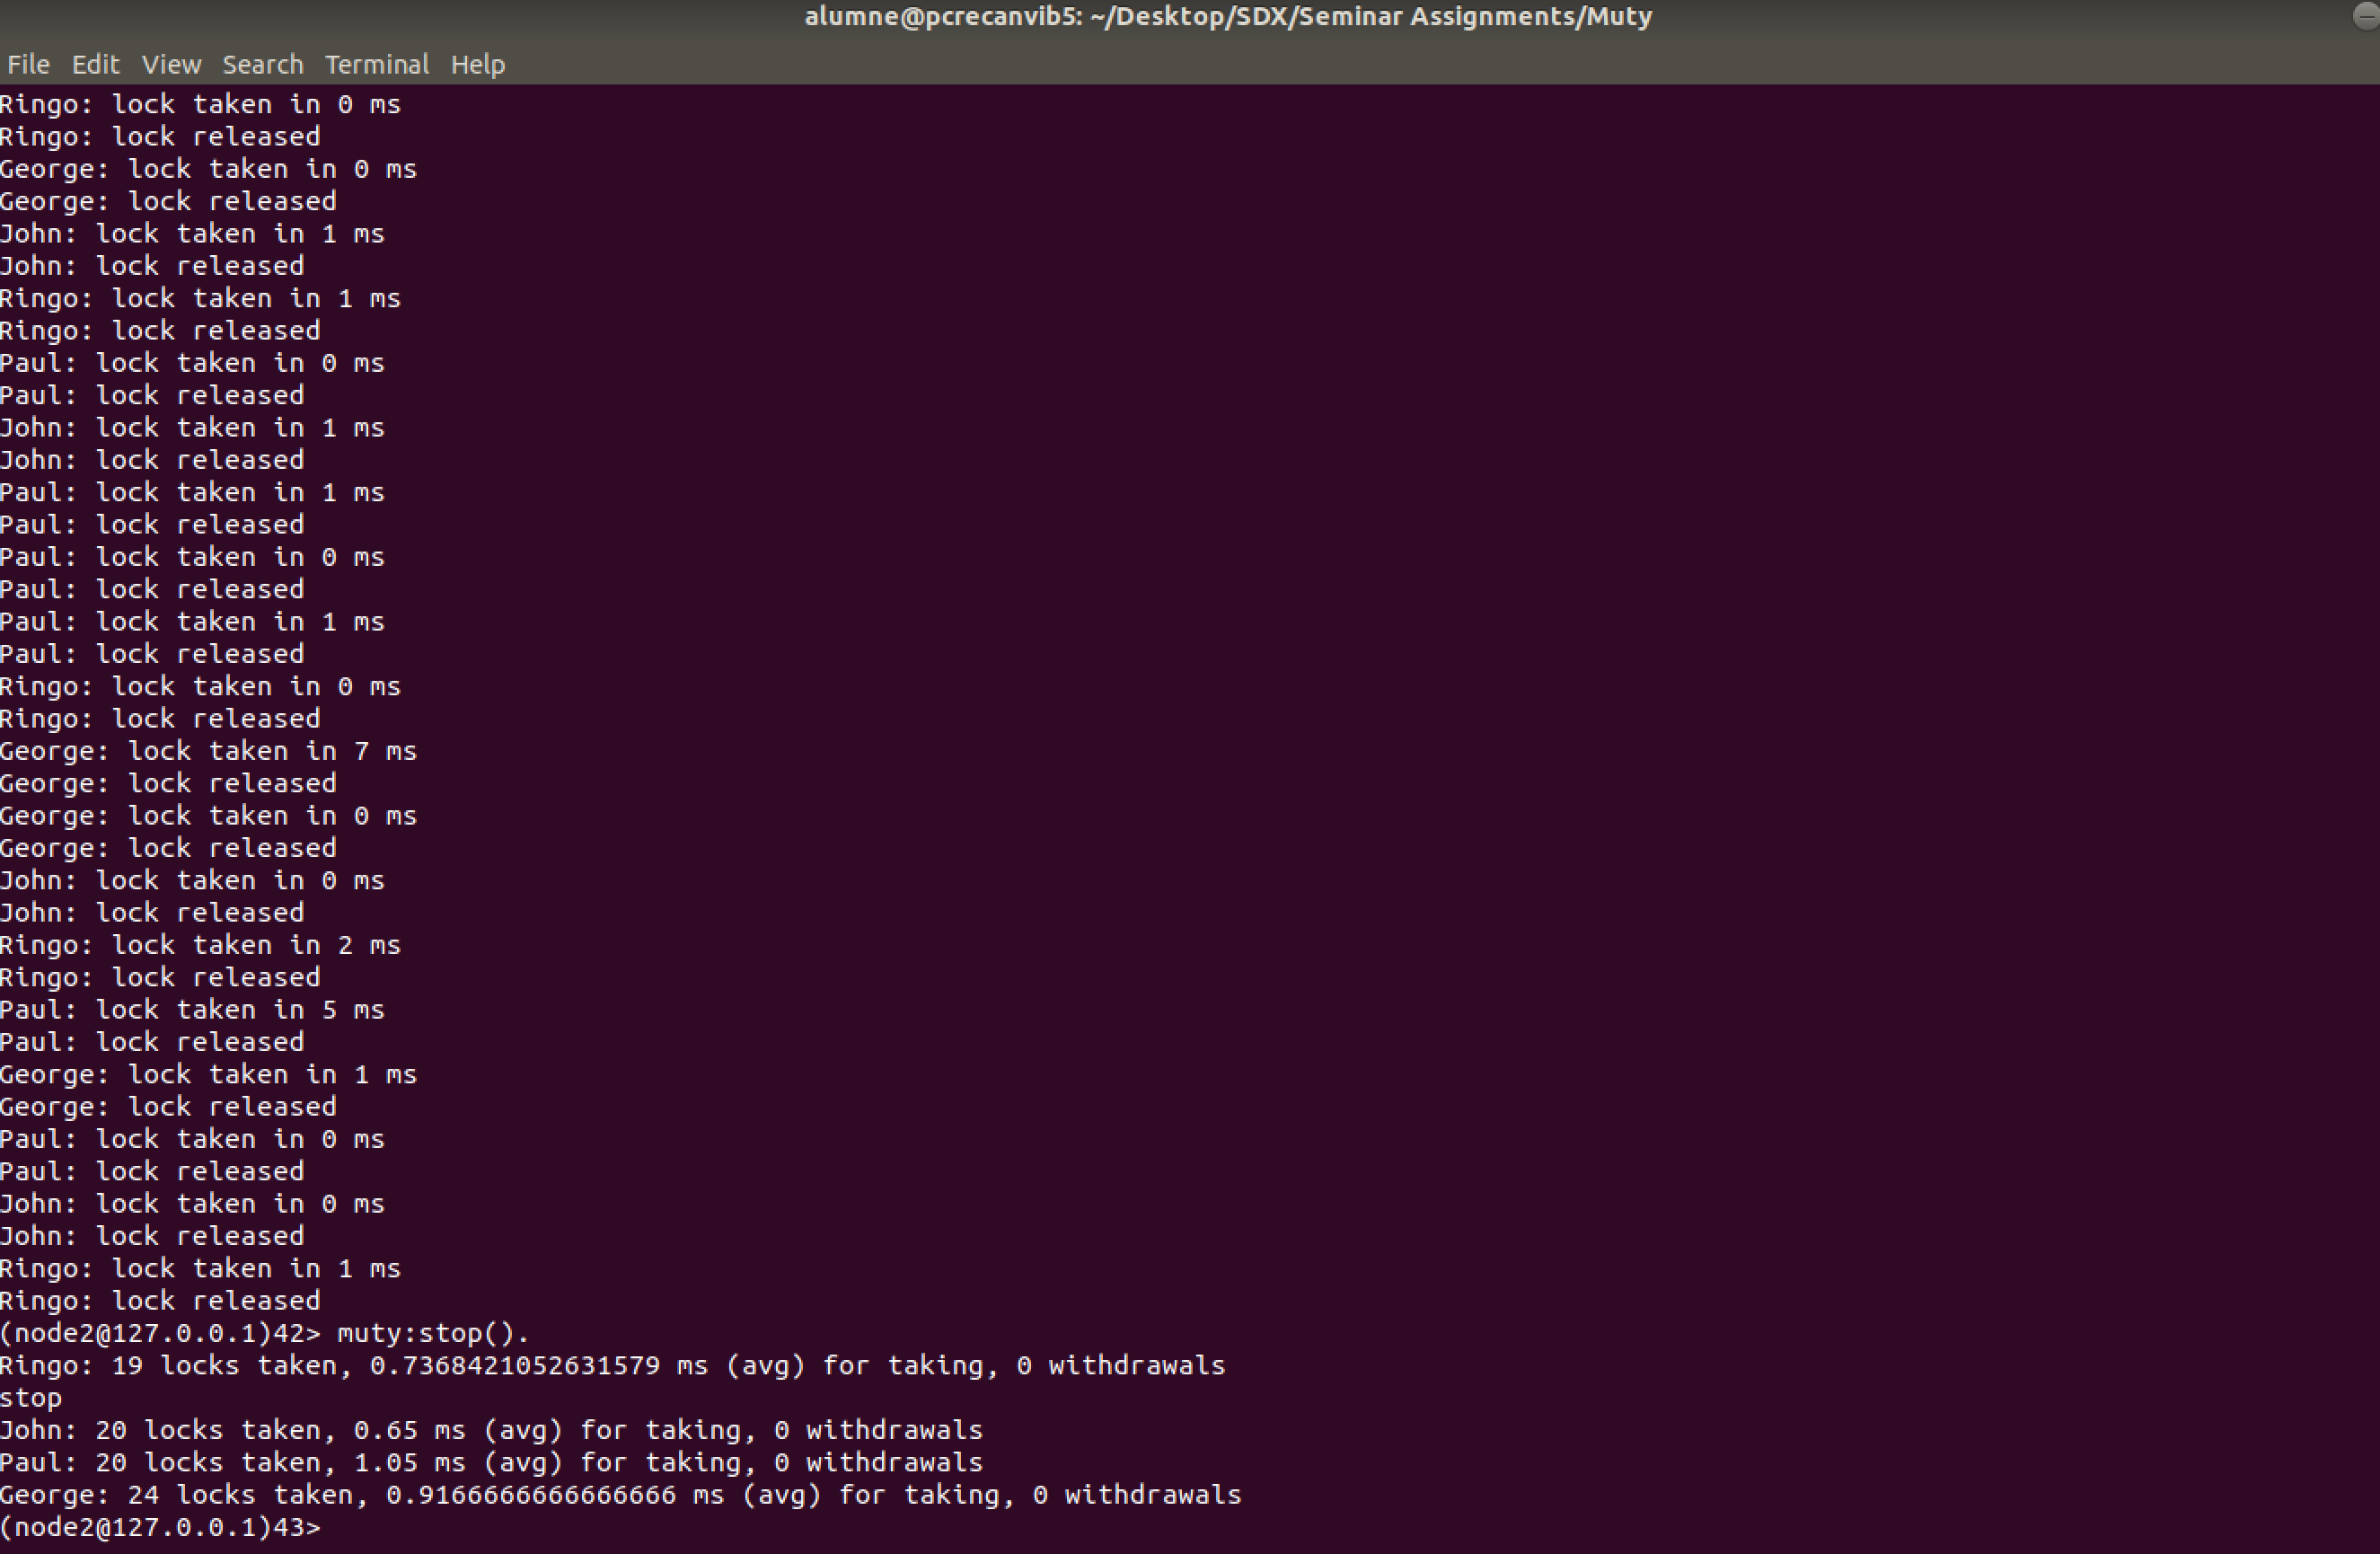
\includegraphics[width=\textwidth]{lamp-2}

\end{enumerate}

\newpage
\section{Open questions}
\paragraph[bold]{4.1 The architecture}
\item What is the behavior of this lock when you increase the risk of a conflict?


\paragraph[bold]{4.2 Resolving deadlock}
\item Justify how your code guarantees that only oneprocess is in the critical section at any time.

\item What is the main drawback of lock2 implementation?

\paragraph[bold]{4.3 Lamport's time}
\item Note that the workers are not involved in the Lam-port’s clock.  According to this, would it be possible that a worker is givenaccess to a critical section prior to another worker that issued a request toits lock instance logically before (assuming happened-before order)?


\newpage
\section{Personal opinion}
\end{document}
